In 2015 the United Nations set up the 17 Sustainable Development Goals. These outline global political actions that must be taken to achieve a better and more sustainable future for all. Each Goal describes a political, economical, social or environmental issue and a set of guidelines on what should be accomplished in that field by the year 2030.\\

The 7th Sustainable Development Goal\cite{UNdev_goal7} aims to ensure access to affordable, reliable, sustainable and modern energy for all. It has subgoals which incentivize improving the energy effiency in all applications, to minimize excessive energy use. When considering the global scale of transportation of perishable goods, it is apparent that improving the energy efficiency of refrigeration trailers (hereinafter reefer trailers) is an important contribution to improve energy efficiency and reduce global energy consumption. \\

%improving the energy efficiency of the shipping is vital

The second Sustainable Development Goal \cite{UNdev_goal2} aims among others to achieve food security. As reefer trailers are used extensively for transportation of fresh foods across the globe, they are one of the backbones in infrastructure of food security. The energy efficiency of reefer trailers is correlated to the cost of transportation of fresh foods. Hence improvement of energy efficiency of reefer trailers can lower the costs of transportation of fresh foods which in the end can lower the price of fresh foods. More affordable fresh foods will help support food security for people globally.\\
   

This project deals with modeling and control of a reefer trailer whose purpose is to maintain specific temperatures inside a box for the transportation of cargo. Many types of products are considered perishable and require  a temperature-controlled environment. Examples other than fresh foods includes frozen food, produce, medical supplies (including vaccines), and electronics. This further highlights the need for high quality and energy efficient temperature-controlled transportation options. \\
While reefer \textit{containers} are used in shipping, reefer \textit{trailers} are necessary when transporting goods to and from central distribution centers. A typical scenario would be from a production facility to a distribution center where the goods are repackaged and shipped to another distribution center the end users. The reefer trailers come into play again from the recieving distribution center,  where it carries out the transportation to e.g. the grocery store. A picture of the reefer trailer used in the project can be seen in \cref{fig:trailer_picture}

\begin{figure}[h]
	\centering
	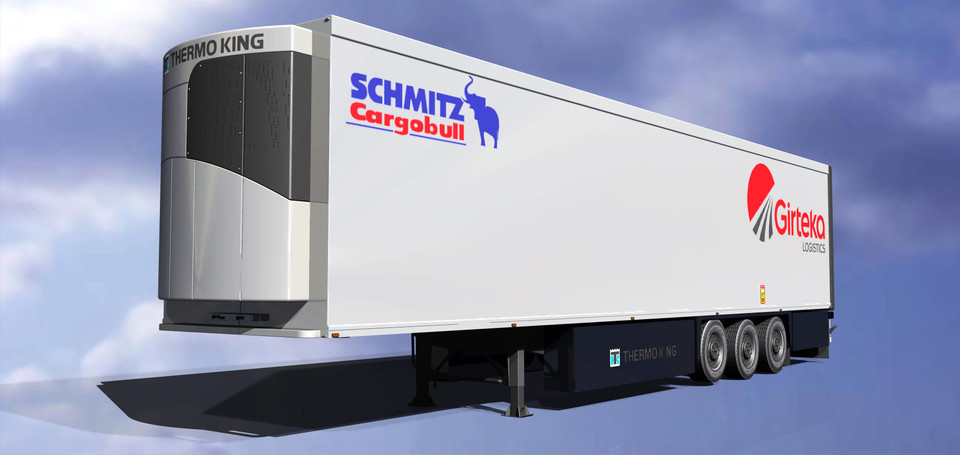
\includegraphics[width = 0.55\linewidth]{Graphics/3d_draw_trailer.jpg}
	\caption{Picture of a Schmitz Cargobull reefer trailer with a cooling unit from Thermo King.}
	\label{fig:trailer_picture}
\end{figure}

Unlike reefer containers, reefer trailers utilize a battery as the main power supply due to the limited power delivery of the trucks they are hooked upon. Efficiency is therefore of great importance as this allows for not only greater transportation distances but also a possible reduction of the battery pack size, which is appealing because of their high cost.

The purpose of a reefer trailer can both be to to maintain the temperature of its cargo and to actually cool it down. The former would typically be the case when transporting goods from distribution centers to end users, where the goods are kept at appropriate temperatures in the distribution center. It is thus expected that cargo is pre-cooled to around the desired transportation temperature before being loaded.
The former would be the case when transporting goods from a production facility (e.g. a plantation) to a distribution center, where the the temperature of the goods could be around ambient temperature.\\

A desired temperature is reached by cooling down air which is circulated between the cargo box and the refrigeration unit. An illustration of the air flows and heat flows can be seen in \cref{fig:trailer_airflow}. The circulated air extracts heat from the cargo, convection heat and occasionally heat that enters the trailer when the doors are opened.

The refrigeration unit is situated at the front of the trailer where all components besides sensors are located. Inside the refrigeration unit a refrigerant is moved between a low pressure side that extracts heat from the returned circulated air, and a high pressure side that transfers heat to ambient air. 

\begin{figure}[h]
	\centering
	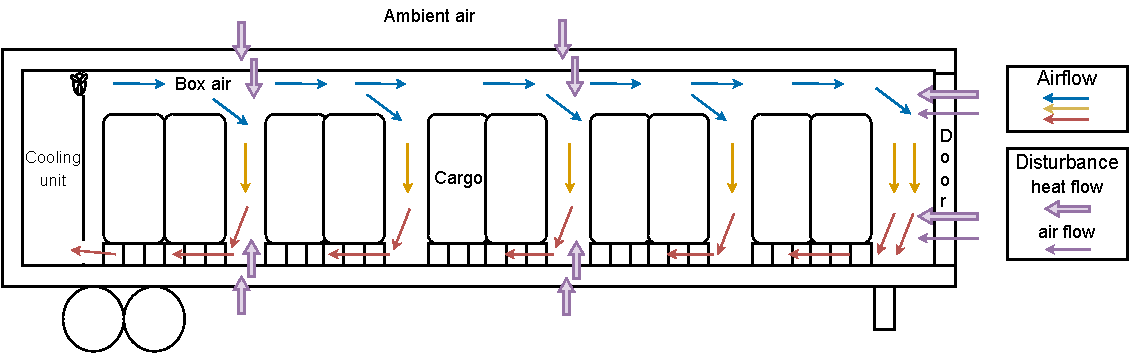
\includegraphics[width = 0.8\linewidth]{Graphics/Trailer_airflow.pdf}
	\caption{Diagram of airflow inside trailer box including disturbances}
	\label{fig:trailer_airflow}
\end{figure}

%The main disturbances in the system are:
%\begin{itemize}
%	\item The air that blows in when the door is opened
%	\item The continuous convection heat transfer from the outside to the inside of the box.
%	\item Cargo temperature
%\end{itemize} 
This project is executed in corporation with BITZER Electronics A/S as a 2nd (8th) semester project of the Masters Program in Control and Automation at Aalborg University.


BITZER is a company that \todo[inline]{Add text about BITZER}


BITZER supplies a high fidelity model of the reefer trailer along with other relevant documentation on the system. Furthermore Kresten Sørensen from BITZER has offered counseling throughout the project.

The purpose of this project is to formulate and implement a MIMO controller for the given reefer trailer. Most control paradigms implemented in reefer systems today are still based on classical control theory such as the PID controller. The control scheme currently in place from BITZER is also made from several coupled PID controllers. BITZER wants to explore the possibility of implementing more modern control in the form of some MIMO controller, which could potentially reduce energy consumption while maintaining a proper temperature of the cargo.

The construction of a controller will require a model of the refrigeration system and as such a controller model will be made to this end. In order to evaluate the controller performance it will be benchmarked against the control scheme currently in place at BITZER.